%going to re organize: place the scenario (methods and all) after the results of the official a priori results
\chapter{Power Analysis} \label{ch:poweranslysis}

\section{Methods}

\subsection{Introduction}

The Park-wide park-wide stream survey has used elevation bands to further organize sites since its conception.
The trend analysis of this paper along with past analyses have all determined trends within these bands , and the lack of high elevation sites brings the power of these trends into question.
Power is the probability of correctly rejecting the false null hypothesis and is increased by minimizing error.
An inherent amount of error comes with the hypothesis test of trend analysis preformed in \autoref{ch:TA}.
Trend analysis tests the hypothesis that a trend exists in the data, which makes the null hypothesis one of no trend or a coefficient that equals zero.
The error here is defined as type II error or $\beta$ and can be seen in \autoref{tab:Hypotests}.
$\beta$ describes the failure to reject a false null hypothesis or in the case of this paper a failure to reject a "no trend" conclusion when there really is one.
The opposite of $\beta$ is the probability that a "no trend" conclusion will be rejected when a trend exists and is called the power of the test.
A trend line with a power of 1.00 indicates a 100$\%$ chance that the calculated slope is not zero, a power of .50 means there is a 50$\%$ chance that the calculated slope might not exist.
Power indicates the reliability of the trends that are important in determining the health of streams in the GRSM.

% Table generated by Excel2LaTeX from sheet 'Hypothesis tests'
\begin{table}[H]
  \centering
  \caption{Hypothosis test results \citep{helsel1992statistical}}
    \begin{tabular}{c|c|c|c}
    \toprule
                                                                                              \multicolumn{2}{c}{} 	                                                                         & \multicolumn{2}{c}{Unknown True Situation} 	                                                                                                                                                                                                                         \\\cline{3-4} 
                                                                                                    \multicolumn{2}{c}{}                                                                          & H$_0$ is true                                                                                                                                                                      & H$_0$ is false                                                                                                                           \\
\midrule
\multirow{6}{*}{\begin{sideways}Decision\end{sideways}}    &\multirow{2}{2cm}{Fail to reject H$_0$}          & \multirow{2}{5.5cm}{Correct decision\\ Prob(correct decision) = 1-$\alpha$}                                                                    & \multirow{2}{5.5cm}{Type II error\\ Prob(Type II error) = $\beta$}                                        \\
	                                                                                         &\multirow{2}{2cm}[-1.5cm]{Reject H$_0$}        &\multirow{2}{5.5cm}[-1.5cm]{Type I error\\ Prob (Type I error) = $\alpha$ \\\textbf{Significance level}}                                  &\multirow{2}{5.5cm}[-1.5cm]{Correct decision\\ Prob (correct decision) = 1-$\beta$\\ \textbf{Power}} \\\cline{2-4}
&&&\\
&&&\\
&&&\\
    \bottomrule
    \end{tabular}%
  \label{tab:Hypotests}%
\end{table}%


Power analysis refers to both  post hoc and a priori analyses, in this paper both are completed with the help of the statistical program G*power.
It can compute both analyses for many different statistical tests, power analysis for regression was used here \citep{faul2009statistical}.
All 144 trend lines from \autoref{ch:TA} were evaluated using a post hoc analysis and also an a priori analysis to project the current park-wide stream survey program into the future.
The two different power analyses are a rearrangement of the same method and have many similarities, but the post hoc analysis determines power while the a priori analysis determines number of observations.
Post hoc of course is Latin for "after this" and is used to denote a power analysis after the completed trend analysis from \autoref{ch:TA}.
A priori is Latin for "from the earlier" and specifies a power analysis used to set a desired power and calculate the number of observations from it.

A post hoc analysis was preformed for both of the Julian date coefficient tables from the step-wise equations in \autoref{sec:swjdc} and the time variable equations in \autoref{sec:tvjdc}, and are presented here in \autoref{sec:posthoc}.
In contrast to the post hoc analysis the a priori analysis only needs to be calculated for each of the four dependent variables.
This is because for each analysis the three inputs (number of predictors, power, and ES) remain the same for each variable.
The front analysis is only for one chosen power, and one chosen ES but G*power will create a power graph which plots each power and the number of observations it needs.
But this is where the analysis in G*power ends and the results must be applied to the park-wide stream survey to get more specific results.
This was accomplished in Excel, where the number of observations given by the power analysis were divided among the elevation bands.
In this way elevation bands with many sites can be shown to contain more observations over time than necessary and elevation bands with lower amounts of sites are shown to need more observations for the same time period.

\subsection{Procedures}

The most general power analysis methods originate from Jacob Cohen, who outlined his approach in" A Power Primer" \citep{cohen1992power}.
Cohen displayed ways to calculate the power for eight different tests the last of which is the F test for multiple and multiple partial correlation, which can be used for regression.
The different tests are represented by their differences in calculating ES, which is described by Cohen as the probability to find a significant result \citep{cohen1992power}.
The equation for the ES of a regression model presented by Cohen is equal to the correlation coefficient divided by one minus the correlation coefficient.
\begin{equation} \label{eq:ES}
    ES = {adj. r^2 \over {1-adj. r^2}}
\end{equation}
This equation can be described as the ratio of explained to unexplained variation for the regression model.
For the post hoc analysis this equation will be used to calculate a specific ES for each model from both methods of equations used for trend analysis in \autoref{sec:swjdc} and \autoref{sec:tvjdc}.
The ES calculation is completed by G*power after inputting the correlation coefficient (adj. r$^2$).

\subsubsection{Post hoc}

G*power uses ES along with the $\alpha$ (.05) used for the regression model, the number observations, and number of predictors in the model to output the power of the F test for regression.
This power will be between 0 and 1.00 and will be the power acquired by the models using past data and a calculated ES.
With post hoc analysis, three of these inputs are passed from the output of the trend analysis: number of observations (N), adjusted r$^2$ and number of predictors.
The fourth input is ES or effect size which is calculated by G*power before the study.
A priori analysis also requires an ES value but it is chosen, instead of calculated, along with the power.
Just like the post hoc analysis the number of predictors is still needed for the a priori analysis and taken from the number of predictors given in the step-wise analysis in \autoref{tab:stepwiseeq}.

\subsubsection{A priori}

The a priori analysis is more conditional than the straight forward calculations for the post hoc analysis.
Instead of outputting a power value like the post hoc analysis, G* power will compute the number of observations for a given scenario. 
The inputs for this study are $\alpha$ (.05), desired power, number of predictors, and ES.
All of these inputs can be changed or manipulated based on the anticipated outcome.
For this analysis the assumption was made that the same trend analysis as the one completed in \autoref{ch:TA} would be attempted in the future.
Based on this assumption the same step-wise equations constructed in \autoref{tab:stepwiseeq} can be used to help chose the number of predictors and $\alpha$.

The most encompassing way to present an a priori analysis is through a power graph.
The power graphs plot power on the y-axis and number of observations on the x-axis.
Using this as a tool a planner can choose a desired power and get the corresponding number of observations.

Choosing an ES value and desired power will be a matter of convention.
To make choosing the ES value easier Cohen has defined small, medium, and large ES values for each of the eight tests described in \citet{cohen1992power}.
Concerning the multiple and multiple partial correlation test he decided on .02, .15, and .35 respectively.
All of these ES values can be graphed in the power graphs by plotting different ES values as curves on the same plot.
But in order to later determine more efficient site counts per elevation band a best ES value must be chosen.
An ES value of .15 was settled upon after the power graphs for all three conventions per dependent variable were made.
.02 was too small, requiring very high numbers of observations to reach a decent power.
ES values of .35 can acquire small numbers of observations thus achieving a decent power level easier, but the smaller the ES the better.
.15 is less than half of .35 so it minimizes the chances for insignificant results and the numbers of observations are reasonable to reach higher powers.
If no argument can be made for any other desired power then Cohen suggests .80.
This is chosen for its reasonable ratio of Type I error to Type II error which reflects their importance.
If the power is .80 then $\beta=.20$ and $\alpha=.05$ and this makes the Type II error four times as likely as Type I error \citep{cohen1992statistical}.

\section{Results}

\subsection{Post hoc}\label{sec:posthoc}

% Table generated by Excel2LaTeX from sheet 'Post Hoc Power analysis'
\begin{table}[htbp]
  \centering
	\caption{pH Step-Wise Post Hoc Power Analysis Results}
    \begin{tabular}{rrcrrr}
    \toprule
    Set   & Class & N     & Adjusted r$^2$ & Effect Size & Actual Power \\
    \midrule
    \multicolumn{1}{c}{\multirow{6}[1]{*}{\begin{sideways}1993-2002\end{sideways}}} & \multicolumn{1}{c}{1} & \multicolumn{1}{c}{327} & \multicolumn{1}{c}{0.712} & \multicolumn{1}{r}{2.47 } & \multicolumn{1}{c}{1.00 } \\
    \multicolumn{1}{c}{} & \multicolumn{1}{c}{2} & \multicolumn{1}{c}{393} & \multicolumn{1}{c}{0.388 } & \multicolumn{1}{r}{0.63 } & \multicolumn{1}{c}{1.00 } \\
    \multicolumn{1}{c}{} & \multicolumn{1}{c}{3} & \multicolumn{1}{c}{400} & \multicolumn{1}{c}{0.693 } & \multicolumn{1}{r}{2.26 } & \multicolumn{1}{c}{1.00 } \\
    \multicolumn{1}{c}{} & \multicolumn{1}{c}{4} & \multicolumn{1}{c}{121} & \multicolumn{1}{c}{0.205 } & \multicolumn{1}{r}{0.26 } & \multicolumn{1}{c}{0.99 } \\
    \multicolumn{1}{c}{} & \multicolumn{1}{c}{5} & \multicolumn{1}{c}{116} & \multicolumn{1}{c}{0.165 } & \multicolumn{1}{r}{0.20 } & \multicolumn{1}{c}{0.96 } \\
    \multicolumn{1}{c}{} & \multicolumn{1}{c}{6} & \multicolumn{1}{c}{110} & \multicolumn{1}{c}{0.505} & \multicolumn{1}{r}{1.02 } & \multicolumn{1}{c}{1.00 } \\\midrule
    \multicolumn{1}{c}{\multirow{6}[2]{*}{\begin{sideways}2003-2008\end{sideways}}} & \multicolumn{1}{c}{1} & \multicolumn{1}{c}{255} & \multicolumn{1}{c}{0.781 } & \multicolumn{1}{r}{3.57 } & \multicolumn{1}{c}{1.00 } \\
    \multicolumn{1}{c}{} & \multicolumn{1}{c}{2} & \multicolumn{1}{c}{289} & \multicolumn{1}{c}{0.348 } & \multicolumn{1}{r}{0.53 } & \multicolumn{1}{c}{1.00 } \\
    \multicolumn{1}{c}{} & \multicolumn{1}{c}{3} & \multicolumn{1}{c}{299} & \multicolumn{1}{c}{0.663 } & \multicolumn{1}{r}{1.97 } & \multicolumn{1}{c}{1.00 } \\
    \multicolumn{1}{c}{} & \multicolumn{1}{c}{4} & \multicolumn{1}{c}{119} & \multicolumn{1}{c}{0.400 } & \multicolumn{1}{r}{0.67 } & \multicolumn{1}{c}{1.00 } \\
    \multicolumn{1}{c}{} & \multicolumn{1}{c}{5} & \multicolumn{1}{c}{35} & \multicolumn{1}{c}{0.300 } & \multicolumn{1}{r}{0.43 } & \multicolumn{1}{c}{0.74 } \\
    \multicolumn{1}{c}{} & \multicolumn{1}{c}{6} & \multicolumn{1}{c}{97} & \multicolumn{1}{c}{0.317} & \multicolumn{1}{r}{0.46 } & \multicolumn{1}{c}{1.00 } \\\midrule
    \multicolumn{1}{c}{\multirow{6}[2]{*}{\begin{sideways}2009-2012\end{sideways}}} & \multicolumn{1}{c}{1} & \multicolumn{1}{c}{191} & \multicolumn{1}{c}{0.894 } & \multicolumn{1}{r}{8.43 } & \multicolumn{1}{c}{1.00 } \\
    \multicolumn{1}{c}{} & \multicolumn{1}{c}{2} & \multicolumn{1}{c}{212} & \multicolumn{1}{c}{0.606 } & \multicolumn{1}{r}{1.54 } & \multicolumn{1}{c}{1.00 } \\
    \multicolumn{1}{c}{} & \multicolumn{1}{c}{3} & \multicolumn{1}{c}{228} & \multicolumn{1}{c}{0.766 } & \multicolumn{1}{r}{3.27 } & \multicolumn{1}{c}{1.00 } \\
    \multicolumn{1}{c}{} & \multicolumn{1}{c}{4} & \multicolumn{1}{c}{97} & \multicolumn{1}{c}{0.593 } & \multicolumn{1}{r}{1.46 } & \multicolumn{1}{c}{1.00 } \\
    \multicolumn{1}{c}{} & \multicolumn{1}{c}{5} & \multicolumn{1}{c}{29} & \multicolumn{1}{c}{\textbf{0.158 }} & \multicolumn{1}{r}{0.19 } & \multicolumn{1}{c}{0.28 } \\
    \multicolumn{1}{c}{} & \multicolumn{1}{c}{6} & \multicolumn{1}{c}{76} & \multicolumn{1}{c}{0.286} & \multicolumn{1}{r}{0.40 } & \multicolumn{1}{c}{0.99 } \\
    \bottomrule
    \end{tabular}%
  \label{tab:pHSWPHPA}%
\end{table}%


% Table generated by Excel2LaTeX from sheet 'Post Hoc Power analysis'
\begin{table}[htbp]
  \centering
	\caption{ANC Step-Wise Post Hoc Power Analysis Results}
    \begin{tabular}{rrcrrr}
    \toprule
    Set   & Class & N     & Adjusted r$^2$ & Effect Size & Actual Power \\
    \midrule
    \multicolumn{1}{c}{\multirow{6}[1]{*}{\begin{sideways}1993-2002\end{sideways}}} & \multicolumn{1}{c}{1} & \multicolumn{1}{c}{327} & \multicolumn{1}{c}{0.985 } & \multicolumn{1}{r}{65.67 } & \multicolumn{1}{c}{1.00 } \\
    \multicolumn{1}{c}{} & \multicolumn{1}{c}{2} & \multicolumn{1}{c}{392} & \multicolumn{1}{c}{0.603 } & \multicolumn{1}{r}{1.52 } & \multicolumn{1}{c}{1.00 } \\
    \multicolumn{1}{c}{} & \multicolumn{1}{c}{3} & \multicolumn{1}{c}{398} & \multicolumn{1}{c}{0.971 } & \multicolumn{1}{r}{33.48 } & \multicolumn{1}{c}{1.00 } \\
    \multicolumn{1}{c}{} & \multicolumn{1}{c}{4} & \multicolumn{1}{c}{120} & \multicolumn{1}{c}{0.709 } & \multicolumn{1}{r}{2.44 } & \multicolumn{1}{c}{1.00 } \\
    \multicolumn{1}{c}{} & \multicolumn{1}{c}{5} & \multicolumn{1}{c}{116} & \multicolumn{1}{c}{0.760 } & \multicolumn{1}{r}{3.17 } & \multicolumn{1}{c}{1.00 } \\
    \multicolumn{1}{c}{} & \multicolumn{1}{c}{6} & \multicolumn{1}{c}{110} & \multicolumn{1}{c}{0.802} & \multicolumn{1}{r}{4.05 } & \multicolumn{1}{c}{1.00 } \\\midrule
    \multicolumn{1}{c}{\multirow{6}[2]{*}{\begin{sideways}2003-2008\end{sideways}}} & \multicolumn{1}{c}{1} & \multicolumn{1}{c}{255} & \multicolumn{1}{c}{0.996 } & \multicolumn{1}{r}{249.00 } & \multicolumn{1}{c}{1.00 } \\
    \multicolumn{1}{c}{} & \multicolumn{1}{c}{2} & \multicolumn{1}{c}{289} & \multicolumn{1}{c}{0.779 } & \multicolumn{1}{r}{3.52 } & \multicolumn{1}{c}{1.00 } \\
    \multicolumn{1}{c}{} & \multicolumn{1}{c}{3} & \multicolumn{1}{c}{299} & \multicolumn{1}{c}{0.996 } & \multicolumn{1}{r}{249.00 } & \multicolumn{1}{c}{1.00 } \\
    \multicolumn{1}{c}{} & \multicolumn{1}{c}{4} & \multicolumn{1}{c}{119} & \multicolumn{1}{c}{0.779 } & \multicolumn{1}{r}{3.52 } & \multicolumn{1}{c}{1.00 } \\
    \multicolumn{1}{c}{} & \multicolumn{1}{c}{5} & \multicolumn{1}{c}{35} & \multicolumn{1}{c}{0.739 } & \multicolumn{1}{r}{2.83 } & \multicolumn{1}{c}{1.00 } \\
    \multicolumn{1}{c}{} & \multicolumn{1}{c}{6} & \multicolumn{1}{c}{97} & \multicolumn{1}{c}{0.812} & \multicolumn{1}{r}{4.32 } & \multicolumn{1}{c}{1.00 } \\\midrule
    \multicolumn{1}{c}{\multirow{6}[2]{*}{\begin{sideways}2009-2012\end{sideways}}} & \multicolumn{1}{c}{1} & \multicolumn{1}{c}{191} & \multicolumn{1}{c}{0.989 } & \multicolumn{1}{r}{89.91 } & \multicolumn{1}{c}{1.00 } \\
    \multicolumn{1}{c}{} & \multicolumn{1}{c}{2} & \multicolumn{1}{c}{212} & \multicolumn{1}{c}{0.862 } & \multicolumn{1}{r}{6.25 } & \multicolumn{1}{c}{1.00 } \\
    \multicolumn{1}{c}{} & \multicolumn{1}{c}{3} & \multicolumn{1}{c}{228} & \multicolumn{1}{c}{0.997 } & \multicolumn{1}{r}{332.33 } & \multicolumn{1}{c}{1.00 } \\
    \multicolumn{1}{c}{} & \multicolumn{1}{c}{4} & \multicolumn{1}{c}{97} & \multicolumn{1}{c}{0.772 } & \multicolumn{1}{r}{3.39 } & \multicolumn{1}{c}{1.00 } \\
    \multicolumn{1}{c}{} & \multicolumn{1}{c}{5} & \multicolumn{1}{c}{29} & \multicolumn{1}{c}{0.540 } & \multicolumn{1}{r}{1.17 } & \multicolumn{1}{c}{0.96 } \\
    \multicolumn{1}{c}{} & \multicolumn{1}{c}{6} & \multicolumn{1}{c}{76} & \multicolumn{1}{c}{0.809} & \multicolumn{1}{r}{4.24 } & \multicolumn{1}{c}{1.00 } \\
    \bottomrule
    \end{tabular}%
  \label{tab:ANCSWPHPA}%
\end{table}%


% Table generated by Excel2LaTeX from sheet 'Post Hoc Power analysis'
\begin{table}[htbp]
  \centering
	\caption{Nitrate Step-Wise Post Hoc Power Analysis Results}
    \begin{tabular}{rrcrrr}
    \toprule
    Set   & Class & N     & Adjusted r$^2$ & Effect Size & Actual Power \\
    \midrule
    \multicolumn{1}{c}{\multirow{6}[1]{*}{\begin{sideways}1993-2002\end{sideways}}} & \multicolumn{1}{c}{1} & \multicolumn{1}{c}{275} & \multicolumn{1}{c}{0.503 } & \multicolumn{1}{r}{1.01 } & \multicolumn{1}{c}{1.00 } \\
    \multicolumn{1}{c}{} & \multicolumn{1}{c}{2} & \multicolumn{1}{c}{377} & \multicolumn{1}{c}{0.699 } & \multicolumn{1}{r}{2.32 } & \multicolumn{1}{c}{1.00 } \\
    \multicolumn{1}{c}{} & \multicolumn{1}{c}{3} & \multicolumn{1}{c}{365} & \multicolumn{1}{c}{0.359 } & \multicolumn{1}{r}{0.56 } & \multicolumn{1}{c}{1.00 } \\
    \multicolumn{1}{c}{} & \multicolumn{1}{c}{4} & \multicolumn{1}{c}{105} & \multicolumn{1}{c}{0.410 } & \multicolumn{1}{r}{0.69 } & \multicolumn{1}{c}{1.00 } \\
    \multicolumn{1}{c}{} & \multicolumn{1}{c}{5} & \multicolumn{1}{c}{66} & \multicolumn{1}{c}{0.328 } & \multicolumn{1}{r}{0.49 } & \multicolumn{1}{c}{0.98 } \\
    \multicolumn{1}{c}{} & \multicolumn{1}{c}{6} & \multicolumn{1}{c}{81} & \multicolumn{1}{c}{0.871 } & \multicolumn{1}{r}{6.75 } & \multicolumn{1}{c}{1.00 } \\\midrule
    \multicolumn{1}{c}{\multirow{6}[2]{*}{\begin{sideways}2003-2008\end{sideways}}} & \multicolumn{1}{c}{1} & \multicolumn{1}{c}{252} & \multicolumn{1}{c}{0.551 } & \multicolumn{1}{r}{1.23 } & \multicolumn{1}{c}{1.00 } \\
    \multicolumn{1}{c}{} & \multicolumn{1}{c}{2} & \multicolumn{1}{c}{296} & \multicolumn{1}{c}{0.816 } & \multicolumn{1}{r}{4.43 } & \multicolumn{1}{c}{1.00 } \\
    \multicolumn{1}{c}{} & \multicolumn{1}{c}{3} & \multicolumn{1}{c}{297} & \multicolumn{1}{c}{0.637 } & \multicolumn{1}{r}{1.75 } & \multicolumn{1}{c}{1.00 } \\
    \multicolumn{1}{c}{} & \multicolumn{1}{c}{4} & \multicolumn{1}{c}{121} & \multicolumn{1}{c}{0.405 } & \multicolumn{1}{r}{0.68 } & \multicolumn{1}{c}{1.00 } \\
    \multicolumn{1}{c}{} & \multicolumn{1}{c}{5} & \multicolumn{1}{c}{30} & \multicolumn{1}{c}{0.562 } & \multicolumn{1}{r}{1.28 } & \multicolumn{1}{c}{0.98 } \\
    \multicolumn{1}{c}{} & \multicolumn{1}{c}{6} & \multicolumn{1}{c}{98} & \multicolumn{1}{c}{0.832 } & \multicolumn{1}{r}{4.95 } & \multicolumn{1}{c}{1.00 } \\\midrule
    \multicolumn{1}{c}{\multirow{6}[2]{*}{\begin{sideways}2009-2012\end{sideways}}} & \multicolumn{1}{c}{1} & \multicolumn{1}{c}{191} & \multicolumn{1}{c}{0.376 } & \multicolumn{1}{r}{0.60 } & \multicolumn{1}{c}{1.00 } \\
    \multicolumn{1}{c}{} & \multicolumn{1}{c}{2} & \multicolumn{1}{c}{212} & \multicolumn{1}{c}{0.735 } & \multicolumn{1}{r}{2.77 } & \multicolumn{1}{c}{1.00 } \\
    \multicolumn{1}{c}{} & \multicolumn{1}{c}{3} & \multicolumn{1}{c}{228} & \multicolumn{1}{c}{0.598 } & \multicolumn{1}{r}{1.49 } & \multicolumn{1}{c}{1.00 } \\
    \multicolumn{1}{c}{} & \multicolumn{1}{c}{4} & \multicolumn{1}{c}{97} & \multicolumn{1}{c}{0.635 } & \multicolumn{1}{r}{1.74 } & \multicolumn{1}{c}{1.00 } \\
    \multicolumn{1}{c}{} & \multicolumn{1}{c}{5} & \multicolumn{1}{c}{29} & \multicolumn{1}{c}{\textbf{-0.272 }} & \multicolumn{1}{r}{NA} & \multicolumn{1}{c}{NA} \\
    \multicolumn{1}{c}{} & \multicolumn{1}{c}{6} & \multicolumn{1}{c}{76} & \multicolumn{1}{c}{0.881 } & \multicolumn{1}{r}{7.40 } & \multicolumn{1}{c}{1.00 } \\
    \bottomrule
    \end{tabular}%
  \label{tab:NO3SWPHPA}%
\end{table}%


% Table generated by Excel2LaTeX from sheet 'Post Hoc Power analysis'
\begin{table}[htbp]
  \centering
	  \caption{Sulfate Step-Wise Post Hoc Power Analysis Results}
    \begin{tabular}{rrcrrr}
    \toprule
    Set   & Class & N     & Adjusted r$^2$ & Effect Size & Actual Power \\
    \midrule
    \multicolumn{1}{c}{\multirow{6}[1]{*}{\begin{sideways}1993-2002\end{sideways}}} & \multicolumn{1}{c}{1} & \multicolumn{1}{c}{325} & \multicolumn{1}{c}{0.569 } & \multicolumn{1}{r}{1.32 } & \multicolumn{1}{c}{1.00 } \\
    \multicolumn{1}{c}{} & \multicolumn{1}{c}{2} & \multicolumn{1}{c}{390} & \multicolumn{1}{c}{0.766 } & \multicolumn{1}{r}{3.27 } & \multicolumn{1}{c}{1.00 } \\
    \multicolumn{1}{c}{} & \multicolumn{1}{c}{3} & \multicolumn{1}{c}{391} & \multicolumn{1}{c}{0.590 } & \multicolumn{1}{r}{1.44 } & \multicolumn{1}{c}{1.00 } \\
    \multicolumn{1}{c}{} & \multicolumn{1}{c}{4} & \multicolumn{1}{c}{119} & \multicolumn{1}{c}{0.402 } & \multicolumn{1}{r}{0.67 } & \multicolumn{1}{c}{1.00 } \\
    \multicolumn{1}{c}{} & \multicolumn{1}{c}{5} & \multicolumn{1}{c}{116} & \multicolumn{1}{c}{0.566 } & \multicolumn{1}{r}{1.30 } & \multicolumn{1}{c}{1.00 } \\
    \multicolumn{1}{c}{} & \multicolumn{1}{c}{6} & \multicolumn{1}{c}{110} & \multicolumn{1}{c}{0.716 } & \multicolumn{1}{r}{2.52 } & \multicolumn{1}{c}{1.00 } \\\midrule
    \multicolumn{1}{c}{\multirow{6}[2]{*}{\begin{sideways}2003-2008\end{sideways}}} & \multicolumn{1}{c}{1} & \multicolumn{1}{c}{261} & \multicolumn{1}{c}{0.673 } & \multicolumn{1}{r}{2.06 } & \multicolumn{1}{c}{1.00 } \\
    \multicolumn{1}{c}{} & \multicolumn{1}{c}{2} & \multicolumn{1}{c}{298} & \multicolumn{1}{c}{0.893 } & \multicolumn{1}{r}{8.35 } & \multicolumn{1}{c}{1.00 } \\
    \multicolumn{1}{c}{} & \multicolumn{1}{c}{3} & \multicolumn{1}{c}{308} & \multicolumn{1}{c}{0.923 } & \multicolumn{1}{r}{11.99 } & \multicolumn{1}{c}{1.00 } \\
    \multicolumn{1}{c}{} & \multicolumn{1}{c}{4} & \multicolumn{1}{c}{123} & \multicolumn{1}{c}{0.343 } & \multicolumn{1}{r}{0.52 } & \multicolumn{1}{c}{1.00 } \\
    \multicolumn{1}{c}{} & \multicolumn{1}{c}{5} & \multicolumn{1}{c}{37} & \multicolumn{1}{c}{0.884 } & \multicolumn{1}{r}{7.62 } & \multicolumn{1}{c}{1.00 } \\
    \multicolumn{1}{c}{} & \multicolumn{1}{c}{6} & \multicolumn{1}{c}{101} & \multicolumn{1}{c}{0.844 } & \multicolumn{1}{r}{5.41 } & \multicolumn{1}{c}{1.00 } \\\midrule
    \multicolumn{1}{c}{\multirow{6}[2]{*}{\begin{sideways}2009-2012\end{sideways}}} & \multicolumn{1}{c}{1} & \multicolumn{1}{r}{190} & \multicolumn{1}{c}{0.536 } & \multicolumn{1}{r}{1.16 } & \multicolumn{1}{c}{1.00 } \\
    \multicolumn{1}{c}{} & \multicolumn{1}{c}{2} & \multicolumn{1}{c}{212} & \multicolumn{1}{c}{0.887 } & \multicolumn{1}{r}{7.85 } & \multicolumn{1}{c}{1.00 } \\
    \multicolumn{1}{c}{} & \multicolumn{1}{c}{3} & \multicolumn{1}{c}{228} & \multicolumn{1}{c}{0.915 } & \multicolumn{1}{r}{10.76 } & \multicolumn{1}{c}{1.00 } \\
    \multicolumn{1}{c}{} & \multicolumn{1}{c}{4} & \multicolumn{1}{c}{97} & \multicolumn{1}{c}{0.529 } & \multicolumn{1}{r}{1.12 } & \multicolumn{1}{c}{1.00 } \\
    \multicolumn{1}{c}{} & \multicolumn{1}{c}{5} & \multicolumn{1}{c}{29} & \multicolumn{1}{c}{0.658 } & \multicolumn{1}{r}{1.92 } & \multicolumn{1}{c}{1.00 } \\
    \multicolumn{1}{c}{} & \multicolumn{1}{c}{6} & \multicolumn{1}{c}{76} & \multicolumn{1}{c}{0.861 } & \multicolumn{1}{r}{6.19 } & \multicolumn{1}{c}{1.00 } \\
    \bottomrule
    \end{tabular}%
  \label{tab:SO4SWPHPA}%
\end{table}%


% Table generated by Excel2LaTeX from sheet 'Post Hoc Power analysis'
\begin{table}[htbp]
  \centering
  \caption{pH Time Variable Post Hoc Power Analysis Results}
    \begin{tabular}{rrrrrr}
    \toprule
    Set   & Class & N     & Adjusted r$^2$ & Effect Size & Actual Power \\
    \midrule
    \multicolumn{1}{c}{\multirow{6}[1]{*}{\begin{sideways}1993-2002\end{sideways}}} & \multicolumn{1}{c}{1} & \multicolumn{1}{c}{327} & \multicolumn{1}{c}{\textbf{0.047 }} & \multicolumn{1}{c}{0.049 } & \multicolumn{1}{c}{0.93 } \\
    \multicolumn{1}{c}{} & \multicolumn{1}{c}{2} & \multicolumn{1}{c}{393} & \multicolumn{1}{c}{\textbf{0.128 }} & \multicolumn{1}{c}{0.15 } & \multicolumn{1}{c}{1.00 } \\
    \multicolumn{1}{c}{} & \multicolumn{1}{c}{3} & \multicolumn{1}{c}{400} & \multicolumn{1}{c}{\textbf{0.013 }} & \multicolumn{1}{c}{0.01 } & \multicolumn{1}{c}{0.46 } \\
    \multicolumn{1}{c}{} & \multicolumn{1}{c}{4} & \multicolumn{1}{c}{121} & \multicolumn{1}{c}{\textbf{0.059 }} & \multicolumn{1}{c}{0.06 } & \multicolumn{1}{c}{0.61 } \\
    \multicolumn{1}{c}{} & \multicolumn{1}{c}{5} & \multicolumn{1}{c}{116} & \multicolumn{1}{c}{\textbf{0.051 }} & \multicolumn{1}{c}{0.05 } & \multicolumn{1}{c}{0.52 } \\
    \multicolumn{1}{c}{} & \multicolumn{1}{c}{6} & \multicolumn{1}{c}{110} & \multicolumn{1}{c}{\textbf{0.096 }} & \multicolumn{1}{c}{0.11 } & \multicolumn{1}{c}{0.81 } \\\midrule
    \multicolumn{1}{c}{\multirow{6}[2]{*}{\begin{sideways}2003-2008\end{sideways}}} & \multicolumn{1}{c}{1} & \multicolumn{1}{c}{255} & \multicolumn{1}{c}{0.040 } & \multicolumn{1}{c}{0.04 } & \multicolumn{1}{c}{0.78 } \\
    \multicolumn{1}{c}{} & \multicolumn{1}{c}{2} & \multicolumn{1}{c}{289} & \multicolumn{1}{c}{0.061 } & \multicolumn{1}{c}{0.06 } & \multicolumn{1}{c}{0.96 } \\
    \multicolumn{1}{c}{} & \multicolumn{1}{c}{3} & \multicolumn{1}{c}{299} & \multicolumn{1}{c}{\textbf{0.020 }} & \multicolumn{1}{c}{0.02 } & \multicolumn{1}{c}{0.52 } \\
    \multicolumn{1}{c}{} & \multicolumn{1}{c}{4} & \multicolumn{1}{c}{119} & \multicolumn{1}{c}{0.148 } & \multicolumn{1}{c}{0.17 } & \multicolumn{1}{c}{0.97 } \\
    \multicolumn{1}{c}{} & \multicolumn{1}{c}{5} & \multicolumn{1}{c}{35} & \multicolumn{1}{c}{\textbf{-0.069 }} & \multicolumn{1}{c}{NA} & \multicolumn{1}{c}{NA} \\
    \multicolumn{1}{c}{} & \multicolumn{1}{c}{6} & \multicolumn{1}{c}{97} & \multicolumn{1}{c}{0.081 } & \multicolumn{1}{c}{0.09 } & \multicolumn{1}{c}{0.67 } \\\midrule
    \multicolumn{1}{c}{\multirow{6}[2]{*}{\begin{sideways}2009-2012\end{sideways}}} & \multicolumn{1}{c}{1} & \multicolumn{1}{c}{191} & \multicolumn{1}{c}{\textbf{0.028 }} & \multicolumn{1}{c}{0.03 } & \multicolumn{1}{c}{0.47 } \\
    \multicolumn{1}{c}{} & \multicolumn{1}{c}{2} & \multicolumn{1}{c}{212} & \multicolumn{1}{c}{0.052 } & \multicolumn{1}{c}{0.05 } & \multicolumn{1}{c}{0.82 } \\
    \multicolumn{1}{c}{} & \multicolumn{1}{c}{3} & \multicolumn{1}{c}{228} & \multicolumn{1}{c}{\textbf{-0.009 }} & \multicolumn{1}{c}{NA} & \multicolumn{1}{c}{NA} \\
    \multicolumn{1}{c}{} & \multicolumn{1}{c}{4} & \multicolumn{1}{c}{97} & \multicolumn{1}{c}{0.200 } & \multicolumn{1}{c}{0.25 } & \multicolumn{1}{c}{0.99 } \\
    \multicolumn{1}{c}{} & \multicolumn{1}{c}{5} & \multicolumn{1}{c}{29} & \multicolumn{1}{c}{\textbf{0.218 }} & \multicolumn{1}{c}{0.28 } & \multicolumn{1}{c}{0.58 } \\
    \multicolumn{1}{c}{} & \multicolumn{1}{c}{6} & \multicolumn{1}{c}{76} & \multicolumn{1}{c}{0.039 } & \multicolumn{1}{c}{0.04 } & \multicolumn{1}{c}{0.27 } \\
    \bottomrule
    \end{tabular}%
  \label{tab:pHTVPHPA}%
\end{table}%


% Table generated by Excel2LaTeX from sheet 'Post Hoc Power analysis'
\begin{table}[htbp]
  \centering
	  \caption{ANC Time Variable Post Hoc Power Analysis Results}
    \begin{tabular}{rrrrrr}
    \toprule
    Set   & Class & N     & Adjusted r$^2$ & Effect Size & Actual Power \\
    \midrule
    \multicolumn{1}{c}{\multirow{6}[1]{*}{\begin{sideways}1993-2002\end{sideways}}} & \multicolumn{1}{c}{1} & \multicolumn{1}{c}{327} & \multicolumn{1}{c}{\textbf{0.024 }} & \multicolumn{1}{c}{0.02 } & \multicolumn{1}{c}{0.65 } \\
    \multicolumn{1}{c}{} & \multicolumn{1}{c}{2} & \multicolumn{1}{c}{392} & \multicolumn{1}{c}{\textbf{0.189 }} & \multicolumn{1}{c}{0.23 } & \multicolumn{1}{c}{1.00 } \\
    \multicolumn{1}{c}{} & \multicolumn{1}{c}{3} & \multicolumn{1}{c}{398} & \multicolumn{1}{c}{\textbf{0.000 }} & \multicolumn{1}{c}{0.00 } & \multicolumn{1}{c}{0.06 } \\
    \multicolumn{1}{c}{} & \multicolumn{1}{c}{4} & \multicolumn{1}{c}{120} & \multicolumn{1}{c}{\textbf{0.294 }} & \multicolumn{1}{c}{0.42 } & \multicolumn{1}{c}{1.00 } \\
    \multicolumn{1}{c}{} & \multicolumn{1}{c}{5} & \multicolumn{1}{c}{116} & \multicolumn{1}{c}{0.381 } & \multicolumn{1}{c}{0.62 } & \multicolumn{1}{c}{1.00 } \\
    \multicolumn{1}{c}{} & \multicolumn{1}{c}{6} & \multicolumn{1}{c}{110} & \multicolumn{1}{c}{\textbf{0.075 }} & \multicolumn{1}{c}{0.08 } & \multicolumn{1}{c}{0.69 } \\\midrule
    \multicolumn{1}{c}{\multirow{6}[2]{*}{\begin{sideways}2003-2008\end{sideways}}} & \multicolumn{1}{c}{1} & \multicolumn{1}{c}{255} & \multicolumn{1}{c}{\textbf{0.001 }} & \multicolumn{1}{c}{0.00 } & \multicolumn{1}{c}{0.07 } \\
    \multicolumn{1}{c}{} & \multicolumn{1}{c}{2} & \multicolumn{1}{c}{289} & \multicolumn{1}{c}{\textbf{0.081 }} & \multicolumn{1}{c}{0.09 } & \multicolumn{1}{c}{0.99 } \\
    \multicolumn{1}{c}{} & \multicolumn{1}{c}{3} & \multicolumn{1}{c}{299} & \multicolumn{1}{c}{\textbf{-0.003 }} & \multicolumn{1}{c}{NA} & \multicolumn{1}{c}{NA} \\
    \multicolumn{1}{c}{} & \multicolumn{1}{c}{4} & \multicolumn{1}{c}{119} & \multicolumn{1}{c}{\textbf{0.180 }} & \multicolumn{1}{c}{0.22 } & \multicolumn{1}{c}{0.99 } \\
    \multicolumn{1}{c}{} & \multicolumn{1}{c}{5} & \multicolumn{1}{c}{35} & \multicolumn{1}{c}{\textbf{0.337 }} & \multicolumn{1}{c}{0.51 } & \multicolumn{1}{c}{0.93 } \\
    \multicolumn{1}{c}{} & \multicolumn{1}{c}{6} & \multicolumn{1}{c}{97} & \multicolumn{1}{c}{\textbf{0.094 }} & \multicolumn{1}{c}{0.10 } & \multicolumn{1}{c}{0.74 } \\\midrule
    \multicolumn{1}{c}{\multirow{6}[2]{*}{\begin{sideways}2009-2012\end{sideways}}} & \multicolumn{1}{c}{1} & \multicolumn{1}{c}{191} & \multicolumn{1}{c}{\textbf{0.000 }} & \multicolumn{1}{c}{0.00 } & \multicolumn{1}{c}{0.05 } \\
    \multicolumn{1}{c}{} & \multicolumn{1}{c}{2} & \multicolumn{1}{c}{212} & \multicolumn{1}{c}{\textbf{0.056 }} & \multicolumn{1}{c}{0.06 } & \multicolumn{1}{c}{0.85 } \\
    \multicolumn{1}{c}{} & \multicolumn{1}{c}{3} & \multicolumn{1}{c}{228} & \multicolumn{1}{c}{\textbf{-0.002 }} & \multicolumn{1}{c}{NA} & \multicolumn{1}{c}{NA} \\
    \multicolumn{1}{c}{} & \multicolumn{1}{c}{4} & \multicolumn{1}{c}{97} & \multicolumn{1}{c}{\textbf{0.161 }} & \multicolumn{1}{c}{0.19 } & \multicolumn{1}{c}{0.96 } \\
    \multicolumn{1}{c}{} & \multicolumn{1}{c}{5} & \multicolumn{1}{c}{29} & \multicolumn{1}{c}{0.466 } & \multicolumn{1}{c}{0.87 } & \multicolumn{1}{c}{0.98 } \\
    \multicolumn{1}{c}{} & \multicolumn{1}{c}{6} & \multicolumn{1}{c}{76} & \multicolumn{1}{c}{\textbf{0.058 }} & \multicolumn{1}{c}{0.06 } & \multicolumn{1}{c}{0.39 } \\
    \bottomrule
    \end{tabular}%
  \label{tab:ANCTVPHPA}%
\end{table}%


% Table generated by Excel2LaTeX from sheet 'Post Hoc Power analysis'
\begin{table}[htbp]
  \centering
  \caption{Nitrate Time Variable Post Hoc Power Analysis Results}
    \begin{tabular}{rrrrrr}
    \toprule
    Set   & Class & N     & Adjusted r$^2$ & Effect Size & Actual Power \\
    \midrule
    \multicolumn{1}{c}{\multirow{6}[1]{*}{\begin{sideways}1993-2002\end{sideways}}} & \multicolumn{1}{c}{1} & \multicolumn{1}{c}{275} & \multicolumn{1}{c}{0.016 } & \multicolumn{1}{c}{0.02 } & \multicolumn{1}{c}{0.39 } \\
    \multicolumn{1}{c}{} & \multicolumn{1}{c}{2} & \multicolumn{1}{c}{377} & \multicolumn{1}{c}{\textbf{0.017 }} & \multicolumn{1}{c}{0.02 } & \multicolumn{1}{c}{0.55 } \\
    \multicolumn{1}{c}{} & \multicolumn{1}{c}{3} & \multicolumn{1}{c}{365} & \multicolumn{1}{c}{\textbf{-0.004 }} & \multicolumn{1}{c}{NA} & \multicolumn{1}{c}{NA} \\
    \multicolumn{1}{c}{} & \multicolumn{1}{c}{4} & \multicolumn{1}{c}{105} & \multicolumn{1}{c}{\textbf{-0.027 }} & \multicolumn{1}{c}{NA} & \multicolumn{1}{c}{NA} \\
    \multicolumn{1}{c}{} & \multicolumn{1}{c}{5} & \multicolumn{1}{c}{66} & \multicolumn{1}{c}{0.120 } & \multicolumn{1}{c}{0.14 } & \multicolumn{1}{c}{0.68 } \\
    \multicolumn{1}{c}{} & \multicolumn{1}{c}{6} & \multicolumn{1}{c}{81} & \multicolumn{1}{c}{\textbf{0.092 }} & \multicolumn{1}{c}{0.10 } & \multicolumn{1}{c}{0.64 } \\\midrule
    \multicolumn{1}{c}{\multirow{6}[2]{*}{\begin{sideways}2003-2008\end{sideways}}} & \multicolumn{1}{c}{1} & \multicolumn{1}{c}{252} & \multicolumn{1}{c}{0.061 } & \multicolumn{1}{c}{0.06 } & \multicolumn{1}{c}{0.94 } \\
    \multicolumn{1}{c}{} & \multicolumn{1}{c}{2} & \multicolumn{1}{c}{296} & \multicolumn{1}{c}{0.043 } & \multicolumn{1}{c}{0.04 } & \multicolumn{1}{c}{0.87 } \\
    \multicolumn{1}{c}{} & \multicolumn{1}{c}{3} & \multicolumn{1}{c}{297} & \multicolumn{1}{c}{\textbf{-0.003 }} & \multicolumn{1}{c}{NA} & \multicolumn{1}{c}{NA} \\
    \multicolumn{1}{c}{} & \multicolumn{1}{c}{4} & \multicolumn{1}{c}{121} & \multicolumn{1}{c}{0.086 } & \multicolumn{1}{c}{0.09 } & \multicolumn{1}{c}{0.80 } \\
    \multicolumn{1}{c}{} & \multicolumn{1}{c}{5} & \multicolumn{1}{c}{30} & \multicolumn{1}{c}{\textbf{-0.082 }} & \multicolumn{1}{c}{NA} & \multicolumn{1}{c}{NA} \\
    \multicolumn{1}{c}{} & \multicolumn{1}{c}{6} & \multicolumn{1}{c}{98} & \multicolumn{1}{c}{0.046 } & \multicolumn{1}{c}{0.05 } & \multicolumn{1}{c}{0.40 } \\\midrule
    \multicolumn{1}{c}{\multirow{6}[2]{*}{\begin{sideways}2009-2012\end{sideways}}} & \multicolumn{1}{c}{1} & \multicolumn{1}{c}{191} & \multicolumn{1}{c}{\textbf{0.018 }} & \multicolumn{1}{c}{0.02 } & \multicolumn{1}{c}{0.31 } \\
    \multicolumn{1}{c}{} & \multicolumn{1}{c}{2} & \multicolumn{1}{c}{212} & \multicolumn{1}{c}{\textbf{0.011 }} & \multicolumn{1}{c}{0.01 } & \multicolumn{1}{c}{0.22 } \\
    \multicolumn{1}{c}{} & \multicolumn{1}{c}{3} & \multicolumn{1}{c}{228} & \multicolumn{1}{c}{\textbf{-0.004 }} & \multicolumn{1}{c}{NA} & \multicolumn{1}{c}{NA} \\
    \multicolumn{1}{c}{} & \multicolumn{1}{c}{4} & \multicolumn{1}{c}{97} & \multicolumn{1}{c}{\textbf{-0.016 }} & \multicolumn{1}{c}{NA} & \multicolumn{1}{c}{NA} \\
    \multicolumn{1}{c}{} & \multicolumn{1}{c}{5} & \multicolumn{1}{c}{29} & \multicolumn{1}{c}{\textbf{-0.039 }} & \multicolumn{1}{c}{NA} & \multicolumn{1}{c}{NA} \\
    \multicolumn{1}{c}{} & \multicolumn{1}{c}{6} & \multicolumn{1}{c}{76} & \multicolumn{1}{c}{\textbf{-0.016 }} & \multicolumn{1}{c}{NA} & \multicolumn{1}{c}{NA} \\
    \bottomrule
    \end{tabular}%
  \label{tab:NO3TVPHPA}%
\end{table}%


% Table generated by Excel2LaTeX from sheet 'Post Hoc Power analysis'
\begin{table}[htbp]
  \centering
  \caption{Sulfate Time Variable Post Hoc Power Analysis Results}
    \begin{tabular}{rrrrrr}
    \toprule
    Set   & Class & N     & Adjusted r$^2$ & Effect Size & Actual Power \\
    \midrule
    \multicolumn{1}{c}{\multirow{6}[1]{*}{\begin{sideways}1993-2002\end{sideways}}} & \multicolumn{1}{c}{1} & \multicolumn{1}{c}{325} & \multicolumn{1}{c}{0.045 } & \multicolumn{1}{c}{0.05 } & \multicolumn{1}{c}{0.92 } \\
    \multicolumn{1}{c}{} & \multicolumn{1}{c}{2} & \multicolumn{1}{c}{390} & \multicolumn{1}{c}{\textbf{0.009 }} & \multicolumn{1}{c}{0.01 } & \multicolumn{1}{c}{0.32 } \\
    \multicolumn{1}{c}{} & \multicolumn{1}{c}{3} & \multicolumn{1}{c}{391} & \multicolumn{1}{c}{\textbf{-0.004 }} & \multicolumn{1}{c}{ NA} & \multicolumn{1}{c}{NA} \\
    \multicolumn{1}{c}{} & \multicolumn{1}{c}{4} & \multicolumn{1}{c}{119} & \multicolumn{1}{c}{\textbf{-0.016 }} & \multicolumn{1}{c}{NA} & \multicolumn{1}{c}{NA} \\
    \multicolumn{1}{c}{} & \multicolumn{1}{c}{5} & \multicolumn{1}{c}{116} & \multicolumn{1}{c}{\textbf{-0.010 }} & \multicolumn{1}{c}{NA} & \multicolumn{1}{c}{NA} \\
    \multicolumn{1}{c}{} & \multicolumn{1}{c}{6} & \multicolumn{1}{c}{110} & \multicolumn{1}{c}{\textbf{-0.009 }} & \multicolumn{1}{c}{NA} & \multicolumn{1}{c}{NA} \\\midrule
    \multicolumn{1}{c}{\multirow{6}[2]{*}{\begin{sideways}2003-2008\end{sideways}}} & \multicolumn{1}{c}{1} & \multicolumn{1}{c}{261} & \multicolumn{1}{c}{0.043 } & \multicolumn{1}{c}{0.04 } & \multicolumn{1}{c}{0.82 } \\
    \multicolumn{1}{c}{} & \multicolumn{1}{c}{2} & \multicolumn{1}{c}{298} & \multicolumn{1}{c}{0.014 } & \multicolumn{1}{c}{0.01 } & \multicolumn{1}{c}{0.37 } \\
    \multicolumn{1}{c}{} & \multicolumn{1}{c}{3} & \multicolumn{1}{c}{308} & \multicolumn{1}{c}{\textbf{0.006 }} & \multicolumn{1}{c}{0.01 } & \multicolumn{1}{c}{0.18 } \\
    \multicolumn{1}{c}{} & \multicolumn{1}{c}{4} & \multicolumn{1}{c}{123} & \multicolumn{1}{c}{0.023 } & \multicolumn{1}{c}{0.02 } & \multicolumn{1}{c}{0.26 } \\
    \multicolumn{1}{c}{} & \multicolumn{1}{c}{5} & \multicolumn{1}{c}{37} & \multicolumn{1}{c}{\textbf{-0.024 }} & \multicolumn{1}{c}{NA} & \multicolumn{1}{c}{NA} \\
    \multicolumn{1}{c}{} & \multicolumn{1}{c}{6} & \multicolumn{1}{c}{101} & \multicolumn{1}{c}{0.074 } & \multicolumn{1}{c}{0.08 } & \multicolumn{1}{c}{0.64 } \\\midrule
    \multicolumn{1}{c}{\multirow{6}[2]{*}{\begin{sideways}2009-2012\end{sideways}}} & \multicolumn{1}{c}{1} & \multicolumn{1}{c}{190} & \multicolumn{1}{c}{\textbf{0.005 }} & \multicolumn{1}{c}{0.01 } & \multicolumn{1}{c}{0.11 } \\
    \multicolumn{1}{c}{} & \multicolumn{1}{c}{2} & \multicolumn{1}{c}{212} & \multicolumn{1}{c}{\textbf{-0.010 }} & \multicolumn{1}{c}{NA} & \multicolumn{1}{c}{NA} \\
    \multicolumn{1}{c}{} & \multicolumn{1}{c}{3} & \multicolumn{1}{c}{228} & \multicolumn{1}{c}{\textbf{-0.007 }} & \multicolumn{1}{c}{NA} & \multicolumn{1}{c}{NA} \\
    \multicolumn{1}{c}{} & \multicolumn{1}{c}{4} & \multicolumn{1}{c}{97} & \multicolumn{1}{c}{\textbf{-0.011 }} & \multicolumn{1}{c}{NA} & \multicolumn{1}{c}{NA} \\
    \multicolumn{1}{c}{} & \multicolumn{1}{c}{5} & \multicolumn{1}{c}{29} & \multicolumn{1}{c}{\textbf{-0.076 }} & \multicolumn{1}{c}{NA} & \multicolumn{1}{c}{NA} \\
    \multicolumn{1}{c}{} & \multicolumn{1}{c}{6} & \multicolumn{1}{c}{76} & \multicolumn{1}{c}{\textbf{0.007 }} & \multicolumn{1}{c}{0.01 } & \multicolumn{1}{c}{0.08 } \\
    \bottomrule
    \end{tabular}%
  \label{tab:SO4TVPHPA}%
\end{table}%


The results of the post hoc analysis on both the step-wise method trend analyses and the time variable trend analysis are reported in \autoref{sec:posthoc}.
They are broken into the four water quality variables (pH, ANC, NO$_3$, SO$_4$) and divided into the tree time sets (93-02, 03-08, 09-12), and then further divided into the six elevation classes.
Each time trend from \autoref{ch:TA} is described by its number of observations, the adjusted $r^2$, the calculated ES, and finally their observed power.
Of the 72 lines evaluated for power from step-wise trend analysis (\autoref{sec:swjdc}) only eight of them were less than 1.00 and only two were insignificant.
One of the insignificant trends was the trend for Nitrate, set 3, class 5, and along with insignificance, the adjusted $r^2$ was negative (-0.272) and therefore the power could not be found.
The other insignificant trend was pH, set 3, class 5, which received the lowest observed power of .28.

In large dissimilarity from the step-wise trend models, 52 of the 72 trends from the trends using the time variable equations (\autoref{sec:tvjdc}) were insignificant.
Of the 20 significant trends observed powers range from .26 to 1.00, 11 of them are above .80 and 2 are .99 or greater.
The power of an insignificant trend line is useless.

\subsection{A priori}\label{sec:apriori}

\subsubsection{Power graphs}

The traditional presentation for an a priori power analysis is the power graph.
Here the powers  lie on the y-axis while the number of observations lie on the x-axis.
All of the water quality variables and the time model get their own graph except for ANC and NO$_3$, which are the same because they contain the same number of predictors from their step-wise model.
On each graph two curves are plotted representing an ES of either .15 or .35, they all rise from (0, 0) asymptotically towards a power of 1.00.
Despite the similar shapes, the more predictors a model has, the greater number of  observations it needs to reach equal powers, the power graph for sulfate (\autoref{fig:SulfatePowerGraph}) needs almost 30 more samples than the power graph for time variables (\autoref{fig:TVPowerGraph}) to reach a power of .80 with an ES of .15.

\begin{figure}
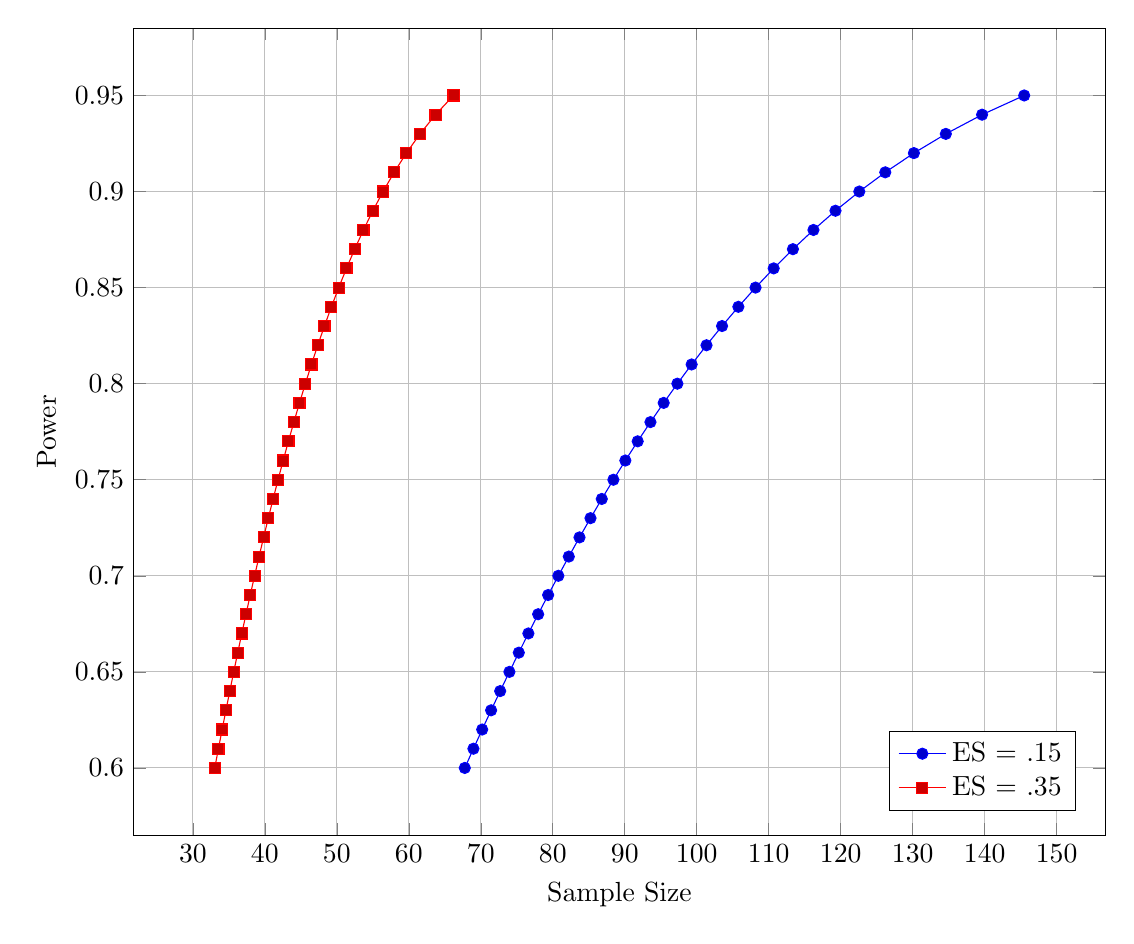
\begin{tikzpicture}
	\begin{axis}[grid=major,xlabel=Sample Size,ylabel=Power,scale=1.8, legend pos = south east]

\addplot coordinates {
(67.7774,	0.60)
(68.9775,	0.61)
(70.196,	0.62)
(71.4343,	0.63)
(72.6936	,0.64)
(73.9752,	0.65)
(75.2807,	0.66)
(76.6116,	0.67)
(77.9697,	0.68)
(79.3569,	0.69)
(80.7752,	0.70)
(82.2269,	0.71)
(83.7145,	0.72)
(85.2407,	0.73)
(86.8085	,0.74)
(88.4213,	0.75)
(90.0829	,0.76)
(91.7974,	0.77)
(93.5697	,0.78)
(95.4052,	0.79)
(97.31,	0.80)
(99.2912,	0.81)
(101.357,	0.82)
(103.517,	0.83)
(105.783,	0.84)
(108.167,	0.85)
(110.686,	0.86)
(113.36,	0.87)
(116.212,	0.88)
(119.273,	0.89)
(122.583	,0.90)
(126.19,	0.91)
(130.165	,0.92)
(134.602,	0.93)
(139.639,	0.94)
(145.49	,0.95)};
\addlegendentry{ES = .15}

\addplot coordinates{
(33.0406	,0.60)
(33.5515	,0.61)
(34.0702	,0.62)
(34.5975	,0.63)
(35.1338,	0.64)
(35.6797	,0.65)
(36.2358,	0.66)
(36.8028,	0.67)
(37.3815,	0.68)
(37.9727,	0.69)
(38.5772,	0.70)
(39.196,	0.71)
(39.8303,	0.72)
(40.481,	0.73)
(41.1496,	0.74)
(41.8375	,0.75)
(42.5462,	0.76)
(43.2777,	0.77)
(44.0338,	0.78)
(44.817,	0.79)
(45.6299,	0.80)
(46.4756,	0.81)
(47.3574,	0.82)
(48.2795,	0.83)
(49.2468,	0.84)
(50.265,	0.85)
(51.3408,	0.86)
(52.4828,	0.87)
(53.7013	,0.88)
(55.0092,	0.89)
(56.423	,0.90)
(57.9647	,0.91)
(59.6634,	0.92)
(61.5598,	0.93)
(63.7132,	0.94)
(66.2148,	0.95)};
\addlegendentry{ES = .35}

\end{axis}
\end{tikzpicture}
\caption[pH Power Graph]{pH Power Graph.  The power is shown as a function of pH}
\label{fig:pHPowerGraph}
\end{figure}

\begin{figure}[htbp]
\centering
\caption[A priori ANC and Nitrate Power Graph]{A priori ANC and Nitrate Power Graph.  The power graphs for ANC and Nitrate are the same because they both have the same number of predictors.}
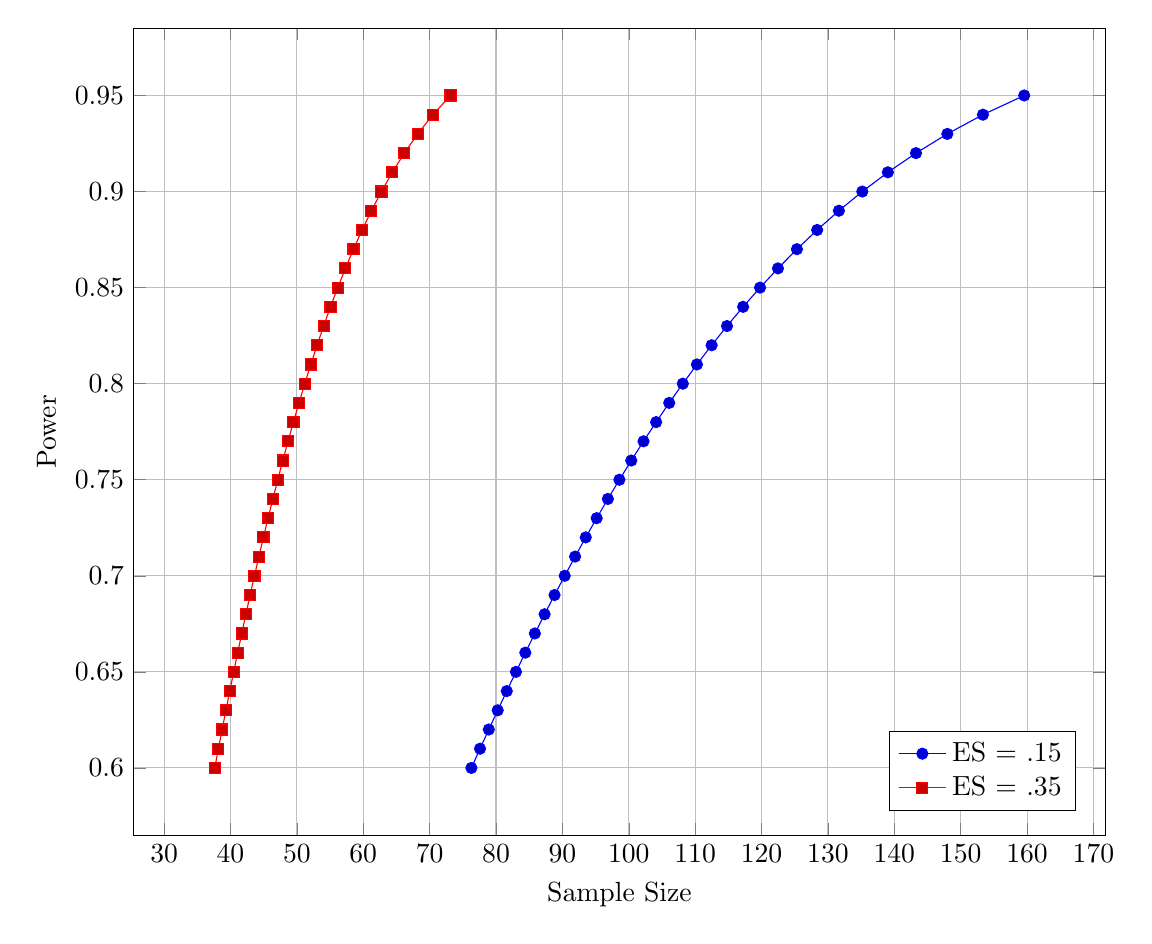
\begin{tikzpicture}
	\begin{axis}[grid=major,xlabel=Sample Size,ylabel=Power,scale=1.8, legend pos= south east] 
\addplot coordinates{
(76.2911	,0.60)
(77.592,	0.61)
(78.9124,	0.62)
(80.2534	,0.63)
(81.6164	,0.64)
(83.0029	,0.65)
(84.4146,	0.66)
(85.853	,0.67)
(87.32,	0.68)
(88.8177,	0.69)
(90.3482,	0.70)
(91.914,	0.71)
(93.5176,	0.72)
(95.162,	0.73)
(96.8504	,0.74)
(98.5864,	0.75)
(100.374,	0.76)
(102.218,	0.77)
(104.122,	0.78)
(106.094,0.79)
(108.139,	0.80)
(110.265,	0.81)
(112.48,	0.82)
(114.795,	0.83)
(117.222,	0.84)
(119.775	,0.85)
(122.471,	0.86)
(125.33,	0.87)
(128.378,	0.88)
(131.647,	0.89)
(135.179,	0.90)
(139.027,	0.91)
(143.263,	0.92)
(147.987,	0.93)
(153.347,	0.94)
(159.566,	0.95)};
\addlegendentry{ES = .15}

\addplot coordinates{
(37.6275,	0.60)
(38.1808,	0.61)
(38.7424,	0.62)
(39.3129,	0.63)
(39.8929,	0.64)
(40.4829,	0.65)
(41.0838,	0.66)
(41.6961,	0.67)
(42.3208,	0.68)
(42.9585,	0.69)
(43.6104,	0.70)
(44.2774,	0.71)
(44.9606,	0.72)
(45.6612,	0.73)
(46.3808,	0.74)
(47.1207,	0.75)
(47.8827,	0.76)
(48.6687,	0.77)
(49.4809,	0.78)
(50.3216,	0.79)
(51.1938,	0.80)
(52.1007,	0.81)
(53.0458,	0.82)
(54.0337,	0.83)
(55.0693,	0.84)
(56.1588,	0.85)
(57.3093,	0.86)
(58.5299,	0.87)
(59.8314,	0.88)
(61.2275	,0.89)
(62.7358,	0.90)
(64.3793,	0.91)
(66.1888,	0.92)
(68.2074,	0.93)
(70.4977,	0.94)
(73.1559,	0.95)};
\addlegendentry{ES = .35}

				
\end{axis}
\end{tikzpicture}
\label{fig:ANCnNPowerGraph}
\end{figure}

\begin{figure}[htbp]
\centering
\caption[A priori Sulfate Power Graph]{A priori Sulfate Power Graph}
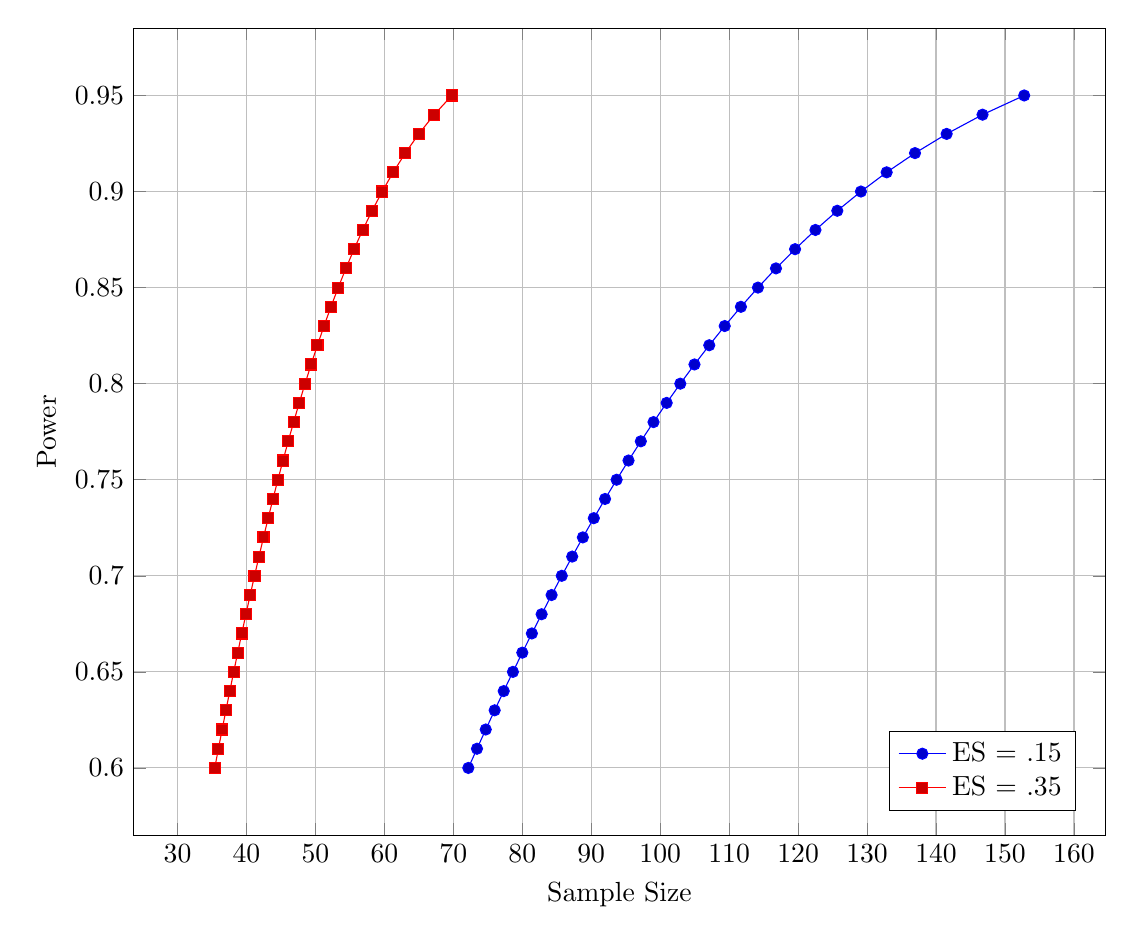
\begin{tikzpicture}
	\begin{axis}[grid=major,xlabel=Sample Size,ylabel=Power,scale=1.8, legend pos = south east] 
\addplot coordinates{
(72.1769,	0.60)
(73.4295,	0.61)
(74.701,	0.62)
(75.9928,	0.63)
(77.3061,	0.64)
(78.6423,	0.65)
(80.0031,	0.66)
(81.3899,	0.67)
(82.8048,	0.68)
(84.2495,	0.69)
(85.7262,	0.70)
(87.2373,	0.71)
(88.7853,	0.72)
(90.373,	0.73)
(92.0036,	0.74)
(93.6806,	0.75)
(95.4078,	0.76)
(97.1895,	0.77)
(99.0308,	0.78)
(100.937,	0.79)
(102.915,	0.80)
(104.971,	0.81)
(107.115,	0.82)
(109.356,	0.83)
(111.705,	0.84)
(114.177,	0.85)
(116.789,	0.86)
(119.559,	0.87)
(122.513,	0.88)
(125.683,	0.89)
(129.108,	0.90)
(132.84,	0.91)
(136.951,	0.92)
(141.538,	0.93)
(146.743,	0.94)
(152.786,	0.95)};
\addlegendentry{ES = .15}

\addplot coordinates{
(35.399	,0.60)
(35.932,	0.61)
(36.4731,	0.62)
(37.0229,	0.63)
(37.582,	0.64)
(38.1509,	0.65)
(38.7303,	0.66)
(39.321,	0.67)
(39.9236,	0.68)
(40.5391,	0.69)
(41.1683,	0.70)
(41.8122,	0.71)
(42.472,	0.72)
(43.1488,	0.73)
(43.8439,	0.74)
(44.5589,	0.75)
(45.2954,	0.76)
(46.0553,	0.77)
(46.8407,	0.78)
(47.6539,	0.79)
(48.4977,	0.80)
(49.3752,	0.81)
(50.29,	0.82)
(51.2464,	0.83)
(52.2493,	0.84)
(53.3046,	0.85)
(54.4195	,0.86)
(55.6024,	0.87)
(56.8641,	0.88)
(58.218,	0.89)
(59.6811,	0.90)
(61.2758,	0.91)
(63.0322,	0.92)
(64.9923,	0.93)
(67.2171,	0.94)
(69.8003,	0.95)};
\addlegendentry{ES = .35}


\end{axis}
\end{tikzpicture}
\label{fig:SulfatePowerGraph}
\end{figure}

\begin{figure}
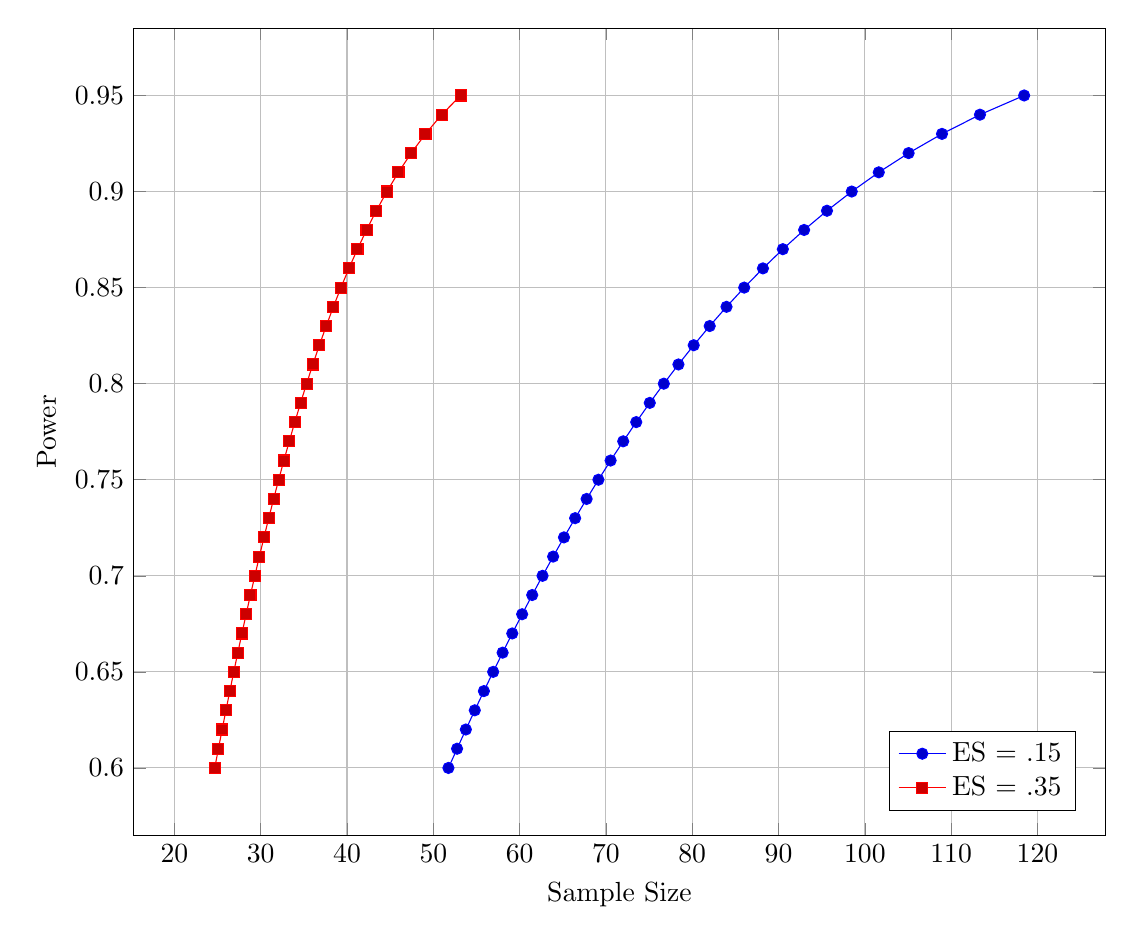
\begin{tikzpicture}
	\begin{axis}[grid=major,xlabel=Sample Size,ylabel=Power,scale=1.8, legend pos= south east] 
\addplot coordinates{
(51.7495	,0.60)
(52.7503,	0.61)
(53.7678,	0.62)
(54.8031,	0.63)
(55.8574,	0.64)
(56.9318,0.65)
(58.0275,	0.66)
(59.1461,	0.67)
(60.289,	0.68)
(61.4578,	0.69)
(62.6543,	0.70)
(63.8806,	0.71)
(65.1387,	0.72)
(66.4311,	0.73)
(67.7605,	0.74)
(69.1297,	0.75)
(70.5422,	0.76)
(72.0015,	0.77)
(73.512,	0.78)
(75.0783,	0.79)
(76.7058,	0.80)
(78.4009,	0.81)
(80.1708,	0.82)
(82.0239,	0.83)
(83.9701,	0.84)
(86.0213,	0.85)
(88.1917,	0.86)
(90.4986,	0.87)
(92.9634,	0.88)
(95.6129,	0.89)
(98.4816,	0.90)
(101.614,	0.91)
(105.072,	0.92)
(108.939,	0.93)
(113.339,	0.94)
(118.46	,0.95)};
\addlegendentry{ES = .15}

\addplot coordinates{
(24.6688	,0.60)
(25.095,	0.61)
(25.5284,	0.62)
(25.9694,	0.63)
(26.4186,	0.64)
(26.8765,	0.65)
(27.3435,	0.66)
(27.8203,	0.67)
(28.3075,	0.68)
(28.8059,	0.69)
(29.3161,	0.70)
(29.8392,	0.71)
(30.3758,	0.72)
(30.9272,	0.73)
(31.4944,	0.74)
(32.0787,	0.75)
(32.6815,	0.76)
(33.3044,	0.77)
(33.9492,	0.78)
(34.6179,	0.79)
(35.3129,	0.80)
(36.0368,	0.81)
(36.7927,	0.82)
(37.5842,	0.83)
(38.4156,	0.84)
(39.292,	0.85)
(40.2194,	0.86)
(41.2052,	0.87)
(42.2586,	0.88)
(43.3911,	0.89)
(44.6174,	0.90)
(45.9568,	0.91)
(47.4353,	0.92)
(49.089,	0.93)
(50.9706,	0.94)
(53.1614,	0.95)};
\addlegendentry{ES = .35}


\end{axis}
\end{tikzpicture}
\caption[Time Variables Power Graph]{Time Variables Power Graph}
\label{fig:TVPowerGraph}
\end{figure}

\subsubsection{A priori manipulation}

\begin{table}[htbp]
		\caption{A priori calculation in G*power when alpha, ES, and power are set to .05, .15, and .80 respectively.}
		\begin{center}
		\begin{tabular}{lcc}
		\hline\noalign{\smallskip}
		 & \multicolumn{1}{l}{Number of predictors} & N \\  \hline\noalign{\smallskip}
		pH & 6 & 98 \\ 
		ANC & 8 & 109 \\ 
		Nitrate & 8 & 109 \\ 
		Sulfate & 7 & 103 \\ 
		Time & 3 & 77 \\  \hline
		\end{tabular}
		\end{center}
		\label{APN}
		\end{table}

The results of the a priori analysis are presented in \autoref{tab:APN} but are inconvenient and require manipulation in order to apply them to the park-wide stream survey.
There are two different ways for the researcher to achieve these results with a focus on time: by adjusting the frequency of collection or by adding sites.
Both methods can be used to quickly acquire enough observations (samples) required by \autoref{tab:APN} to have a powerful trend analysis.
But adding sites is cheaper and can solve the poor elevational distribution of the sites in the park-wide stream survey.

The a priori power analysis can be manipulated to calculate a number of sites per elevation band for the park-wide stream survey in the GRSM.
First, samples per year per elevation band are counted for the 2012 year and will be represented by n.
Next the results from \autoref{tab:APN} are divided by samples per year per elevation band to get the number of years it will take, at the 2012 sampling rate, to reach a power of .80.
\begin{equation} \label{eq:yrs}
    yrs. = {N_a \over n}
\end{equation}
However, in order to get to the number of sites per elevation band needed to reach a power of .80, the years will have to be held constant.
If the future trend analysis is to be completed using the equation with only time variables (instead of the step-wise equations) then 77 samples will need to be collected in one year to reach a power of .80 according to \autoref{tab:APN}.
But if the future trend analysis is to be completed using the step-wise equations from \autoref{tab:stepwiseeq} then at least 109 samples will need to be collected in one year to satisfy the requirements for ANC and NO$_3$.
For the step-wise equations N will be rounded up to 110 and labeled $N_b$.

\begin{table}[htbp]
\caption{samples/year to achieve a power .80}
\begin{center}
\begin{tabular}{lrrrr}
\hline\noalign{\smallskip}
Years & 1 & 2 & 3 & 4 \\ \cline{2-5}\noalign{\smallskip}
Water Quality Variables & 110 & 55 & 37 & 28 \\ 
Time Variables & 77 & 39  & 26  & 19  \\ \hline\noalign{\smallskip}
\end{tabular}
\end{center}
\label{sytaapeighty}
\end{table}

The number of observations required per year per equation are presented in \autoref{tab:sytaapeighty}, which has been calculated out to four years.
Instead of completing the trend analysis after one year, one could wait four years and only need to collect 28 samples per year.
Subtracting the number of samples collected in one year per elevation band in 2012 from the number of samples needed to be collected per year to reach a power of .80 will provide the number of samples needed per elevation band to receive a power of .80 ($N_c$).
\begin{equation} \label{eq:Nc}
    N_c={N_b - n}
\end{equation}
To get an estimation for the number of sites needed per elevation band to achieve a power of .80, the number of samples needed per elevation band to receive a power of .80 ($N_c$) were divided by six which is number of times each site is sampled per year.
\begin{equation}\label{eq:sites}
    \#Sites = {N_c \over 6}
\end{equation}

\begin{table}[htbp]
\caption{Years to acheive a power of .80}
\begin{tabular}{clccccc}
\toprule
\multicolumn{1}{p{2cm}}{Elevation Bands} & \multicolumn{1}{c}{Site \#} & \multicolumn{1}{p{2cm}}{Current n/yr} & pH &\multicolumn{1}{p{1cm}}{ ANC NO$_3$} & SO$_4$ & \multicolumn{1}{p{3cm}}{Time variables} \\  
\midrule
1 & 13 ,23, 24, 30, 479 & 26 & 3.77  & 4.19  & 3.96  & 2.96  \\ 
2 & \multicolumn{1}{p{4cm}}{4, 311, 268, 480, 310, 483, 147, 148, 484} & 34 & 2.88  & 3.21  & 3.03  & 2.26  \\ 
3 & \multicolumn{ 1}{p{4cm}}{114, 481, 482, 149, 66, 492, 137, 293, 270, 493, 485, 144, 224} & \multicolumn{ 1}{c}{62} & \multicolumn{ 1}{c}{1.58 } & \multicolumn{ 1}{c}{1.76 } & \multicolumn{ 1}{c}{1.66 } & \multicolumn{ 1}{c}{1.24} \\ 
4 & 143, 142, 73, 71 & 24 & 4.08  & 4.54  & 4.29  & 3.21  \\ 
5 & 74, 221, 251, 233 & 22 & 4.45  & 4.95  & 4.68  & 3.50  \\ 
6 & 253, 234 & 12 & 8.17  & 9.08  & 8.58  & 6.42  \\  
\bottomrule
\end{tabular}
\label{tab:currentyrsto.80}
\end{table}%needs to be cleaned

This scenario was followed through with both methods of trend lines.
\autoref{tab:currentyrsto.80} records the six elevation bands along with the site numbers that belong to them. 
 In the column labeled, current n per year, the amount of samples collected per elevation band in the year 2012 are tabulated.  
 Then using \autoref{eq:yrs} the number of years needed for each variable to reach a power of .80 is calculated.
Looking at the table there are 26  samples collected in elevation band one in one year.  
In order to compute a trend line for pH using the same step-wise model from \autoref{tab:stepwiseeq} that receives a power of .80,  samples would need to be collected for 3.77 years before the trend line can be computed.   
The longest waiting period is for ANC or NO$_3$ at elevation class six which requires 9.08 years, presumably because they have the highest number of predictors and elevation class six includes only two sites. 

\begin{table}[htbp]
\caption{Necesary sites scenario for water quality variables}
\begin{tabular}{ccccc|ccccc}
\cline{2-9}
\multicolumn{1}{c}{} &   \multicolumn{4}{c}{ \#Samples required} & \multicolumn{4}{c}{\# sites required} \\ \cline{2-9}\noalign{\smallskip}
\multicolumn{1}{p{3cm}}{Elevation Bands}  & 1 yr  & 2 yrs   & 3 yrs    & 4 yrs   & 1 yr   & 2 yrs  & 3 yrs  & 4 yrs\\ \hline\noalign{\smallskip}
1 &  84 & 29 & 11   & 2    & 14 & 5  & 2   & 0 \\ 
2  & 76 & 21 & 3     & -7   & 13 & 4  & 0   & -1 \\ 
3 &  48 & -7  & -25 & -35 & 8   & -1 & -4 & -6 \\
4 &  86 & 31 & 13  & 4     & 14 & 5  & 2  & 1 \\ 
5 &  88 & 33 & 15  & 6     & 15 & 6  & 2  & 1 \\ 
6 &  98 & 43 & 25  & 16   & 16 & 7  & 4  & 3 \\ \hline
\end{tabular}
\label{tab:WQapsenario}
\end{table}%needs to be cleaned

\begin{table}[htbp]
\centering
\caption{Necessary sites scenario for time variables}
\begin{tabular}{ccccc|ccccc}
\toprule
\multicolumn{1}{c}{} &  \multicolumn{4}{c}{ \#Samples required} & \multicolumn{4}{c}{\# sites required} \\ \cline{2-9}\noalign{\smallskip}
\multicolumn{1}{p{3cm}}{Elevation Bands}  & 1 yr   & 2 yrs  & 3 yrs     & 4 yrs   & 1 yr  & 2 yrs & 3 yrs  & 4 yrs \\ \midrule
1 &  51 & 13 & 0 & -7 & 9 & 2 & 0 & -1 \\ 
2 &  43 & 5 & -8 & -15 & 7 & 1 & -1 & -2 \\ 
3 &  15 & -24 & -36 & -43 & 3 & -4 & -6 & -7 \\ 
4 &  53 & 15 & 2 & -5 & 9 & 2 & 0 & -1 \\ 
5 &  55 & 17 & 4 & -3 & 9 & 3 & 1 & 0 \\ 
6 &  65 & 27 & 14 & 7 & 11 & 4 & 2 & 1 \\ \bottomrule
\end{tabular}
\label{tab:TVapsenario}
\end{table}

Tables \autoref{tab:WQapsenario} and \autoref{tab:TVapsenario} correspond to both methods of trend analysis, the step-wise equations and the time variables equations.
Both tables are broken down into two sides, the left side contains number of samples while the right side contains number of sites.
Then each side is arranged by elevation band and calculated out to four years.
\autoref{eq:Nc} is used to calculate the number of samples required and then these numbers are divided by six to get the number of sites.
The numbers on the right side of the tables represent the change to the current number of sites in that elevation band needed to achieve a power of .80 with an ES of .15 using the same models from \autoref{ch:TA}.
In \autoref{tab:WQapsenario} for elevation class 3, 48 more samples need to be collected if a trend line for the water quality dependents with a power of .80 is to be created after one year.  
But if a trend line can wait to be created after two years, then there is a surplus of seven samples per year.  
If four years can be waited there is a surplus of 35 samples which on the right side of the table translates into a surplus of 6 whole site locations per year.

\section{Discussion and Conclusions}

\subsubsection{Post hoc}

\paragraph{Step-wise equations}

By reviewing the results of the post hoc analysis after an a priori analysis has been completed it is easier to see why the results were outstanding for the step-wise equations and awful for the time based equations.
Knowing that an a priori analysis on the step-wise equations will produce a requirement of 110 observations for a power of .80 and an ES of .15 from \autoref{tab:APN}, it can easily be recognized that as the number of observations in the results for the post-hoc power analysis on trends calculated using the step-wise equations (\autoref{sec:posthoc}) decline from 110 the power also declines.
In concert with the large number of observations, the observed ES values are very large compared to the chosen ES of .15 which coincides with the observed powers being close to 1.00.
The large conventional ES given by Cohen is .35 and only 3 of the trend lines analyzed here were below that, all in pH.
And because the ES is a ratio of the adjusted r$^2$ the ES declines as the r$^2$ does, the higher the r$^2$ the better.
But for a calculated ES of .15 the adjusted r$^2$ doesn't need to be very high.
For example, the analyzed trend line for pH in time set 3 elevation class 5 has an adjusted r$^2$ of .158 and the ES is .19, which is larger than .15.
Assuming that a power of .80 and an ES of .15 is ideal, then this post hoc analysis uses too many observations.
One way to have fewer observations would be to use fewer years in the study.
Another way would be to use less sites in the survey.

\paragraph{Time variable based equations}

The two post hoc analyses on the two different models varied considerably.
The differences in powers between the two cannot be caused by a lower number of observations because the number of observations used in both are the same.
But they can be accounted for by the low adjusted r$^2$ values, which are very low for the results for the time variable equations (\autoref{sec:tvjdc}), and leads to the low ES values.
Overlooking the fact that most of the regression models for the time variable analysis are insignificant, most of the powers calculated from \autoref{sec:tvjdc} are not too low.
Of the 20 significant lines eleven have a power equal to or above .80.

\subsubsection{A priori}%it is good that the water quality power graphs are similar because they will all be contained in the same survey.

The a priori power graphs themselves show every possible power and the number of observations needed to achieve it.
However, they are based on the particular step-wise equations that were created using this particular dataset.
Since the step-wise process uses past data to create the equations, every time new data is added the equations could change.
The a priori analysis assumes that these same equations, with the same number of variables, will be used to detect trends in the future.
But even if the number of sites remain the same past this point, the data will still be different.
And if the site numbers do change, such as more sites are added to the upper elevations and sites are removed from the lower elevations, then the step-wise equations are at greater risk of changing.
Then if the number of predictors changes because the data changed this a priori analysis would not be applicable.
A more static set of equations would ease this pressure.

These power graphs can still be used by managers and planners as an educated guess.
After the number of observations for a desired power is determined from the graphs the observations can be placed into the survey with efficiency in mind.
All chosen power and ES values can represent a different scenario.
One such scenario was carried out for a power of .80 and an ES of .15.
Although any value in the power graphs can be chosen these values were chosen as the most efficient. 

The results of this scenario can solve two concerns of the survey, the lack of high elevation sites and the lack of funding.
By following the results in \autoref{tab:WQapsenario}, waiting a minimum of four years before the next trend analysis can lead to the removal of two sites from the survey.
And assuming that cost of the survey is related to the number of sites, then removing sites will save money.
But removing two sites is just the sum difference of a redistribution suggested by the scenario.
In fact, one site should be removed from elevation class 2 and six from elevation class 3.
One site each need to be added to classes 4 and 5 and three sites should be added to class 6.
There are too many sites in the lower elevation classes of 2 and 3 and not enough sites in the higher elevation classes of 4, 5, and 6.
A redistribution of sites is in order.
